\documentclass{article}

\usepackage[utf8]{inputenc}
\usepackage[T1]{fontenc}
\usepackage[greek,english]{babel}
\usepackage{alphabeta}
\usepackage{amsmath}
\usepackage{amssymb}
\usepackage{graphicx}
\usepackage{subcaption}
\usepackage{epstopdf}
\usepackage[margin=1in, paperwidth=7.5in,paperheight=10.5in]{geometry}
\usepackage{hyperref}
\usepackage{paracol}

\newcommand\course{TΗΛ411}
\newcommand\courseName{Ψηφιακή Επεξεργασία Εικόνας}
\newcommand\semester{Χειμερινό 2021}
\newcommand\assignmentNumber{Assignment 3}
\newcommand\studentName{Μαυρογιώργης Δημήτρης}                           
\newcommand\studentNumber{2016030016}

\title{\underline{\textbf{\assignmentNumber}}} 
\author{\textsc{\textbf{Όνομα:}}  \studentName\\
		\textsc{\textbf{ΑΜ:}}  \studentNumber\\
		\course \ - \courseName\\ 
		\textsc{Πολυτεχνείο Κρήτης}
}
\date{\today}
\begin{document}
	\maketitle

\section*{Introduction}
	Ο σκοπός της 3ης εργαστηριακής άσκησης είναι να δημιουργήσουμε μία Γκαουσιανή πυραμίδα, ώστε να αποσυνθέσουμε μία εικόνα σε διάφορα επίπεδα. Επιπλέον, έπρεπε να δημιουργήσουμε την Λαπλασιανή πυραμίδα υπολογίζοντας τις διαφορές των επιπέδων και διευρύνοντας όσα επίπεδα χρειάζεται. Τέλος, χρησιμοποιώντας τα κατάλληλα επίπεδα της Γκαουσιανής και Λαπλασιανής και αθροίζοντας, έπρεπε να επανασυνθέσουμε την αρχική εικόνα.

\section*{Implementation}
	Αρχικά, δημιουργήθηκε με τη συνάρτηση fspecial του Matlab ένα Gaussian φίλτρο 5x5 με τυπική απόκλιση σ = 1. Στη συνέχεια, έγινε η συνέλιξη της εικόνας "cameraman.tif" με το φίλτρο χρησιμοποιώντας τη συνάρτηση imfilter και downsample με παράμετρο scale 1/2 με τη χρήση της συνάρτησης imresize. Τέλος, επαναλήφθηκε η παραπάνω διαδικασία άλλες τέσσερις φορές προκειμένου να αποσυντεθεί η εικόνα και να κατασκευαστεί η επιπέδου 5 Gaussian πυραμίδα.\\
	
	\noindent
	Έπειτα, ο υπολογισμός της Laplacian πυραμίδας, έγινε αφαιρώντας δύο διαδοχικά επίπεδα της Gaussian πυραμίδας, αφού πρώτα έγινε upsample στις εικόνες που είχαν υποστεί downsample για να έχουν το ίδιο μέγεθος.\\
	
	\noindent
	Τέλος, για την ανακατασκευή της εικόνας, συνδυάστηκαν οι δύο πυραμίδες που δημιουργήθηκαν. Πιο συγκεκριμένα, για ένα συγκεκριμένο επίπεδο, εκτός από το πέμπτο επίπεδο που είναι ίδιο στη Laplacian και Gaussian, αθροίστηκαν δύο διαδοχικά επίπεδα, αφού προηγουμένως έγινε upsample στις εικόνες που είχαν γίνει downsampled. \\
	
\section*{Results}
	Στην Gaussian πυραμίδα βλέπουμε ότι καθώς ανεβαίνουμε επίπεδα, η εικόνες αντισταθμίζονται χρησιμοποιώντας το Gaussian φίλτρο και γίνονται πιο θαμπές, επειδή με το low-pass φίλτρο που χρησιμοποιήθηκε εξασθένισαν οι υψηλές συχνότητες. Παράλληλα, βλέπουμε ότι εξαιτίας της υποδειγματοληψίας, η ανάλυση των εικόνων μειώνεται στο μισό κάθε φορά. \\
	
	\pagebreak
	\noindent
	Όσον αφορά την κατασκευή της Laplacian πυραμίδας, είναι πολύ παρόμοια με την πυραμίδα Gauss, μόν που σε κάθε επίπεδο αποθηκεύει την εικόνα της διαφοράς των θολών εκδόσεων μεταξύ διαδοχικών επιπέδων της πυραμίδας Gauss. Μόνο το τελευταίο επίπεδο δεν είναι μια εικόνα διαφοράς, γεγονός που επιτρέπει την ανακατασκευή της αρχικής εικόνας χρησιμοποιώντας τις εικόνες από τα υψηλότερα επίπεδα.\\
	
	\noindent
	Τέλος, όσον αφορά την ανακατασκευασμένη εικόνα, παρατηρούμε ότι με το συνδυασμό των δύο πυραμίδων προέκυψε ακριβώς η αρχική εικόνα όπως ήταν πριν την επεξεργασία. Για τη σύγκριση της αρχικής με την τελική εικόνα χρησιμοποιήθηκε και o δείκτης MSE που μέσω της συνάρτησης immse του Matlab υπολογίστηκε 0, γεγονός που δείχνει ότι δεν υπήρξε καθόλου μεταβολή κατά την επεξεργασία της εικόνας.
	\begin{figure}[h!]
		\centering
		\begin{subfigure}[t]{0.5\textwidth}
			\centering
			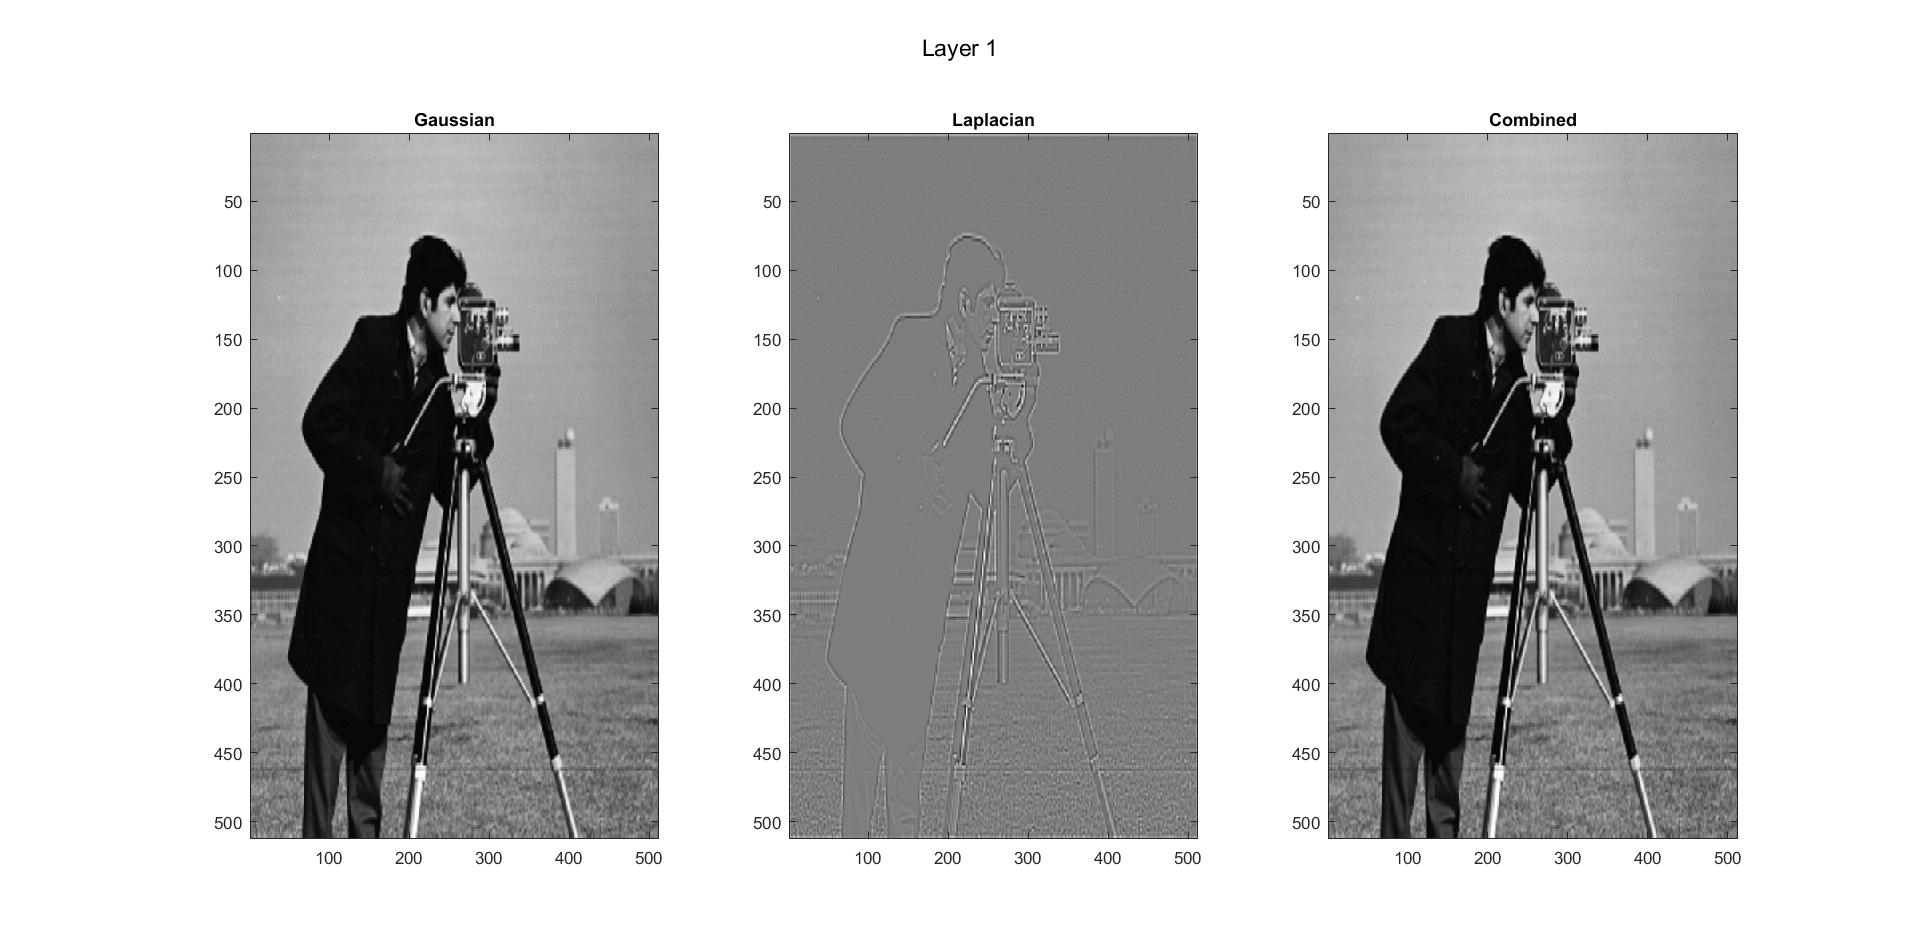
\includegraphics[width=\linewidth]{./output_images/layer_1.jpg}
			\caption{Gaussian and Laplacian pyramid and their compination - Layer 1}
		\end{subfigure}%
		~
		\begin{subfigure}[t]{0.5\textwidth}
			\centering
			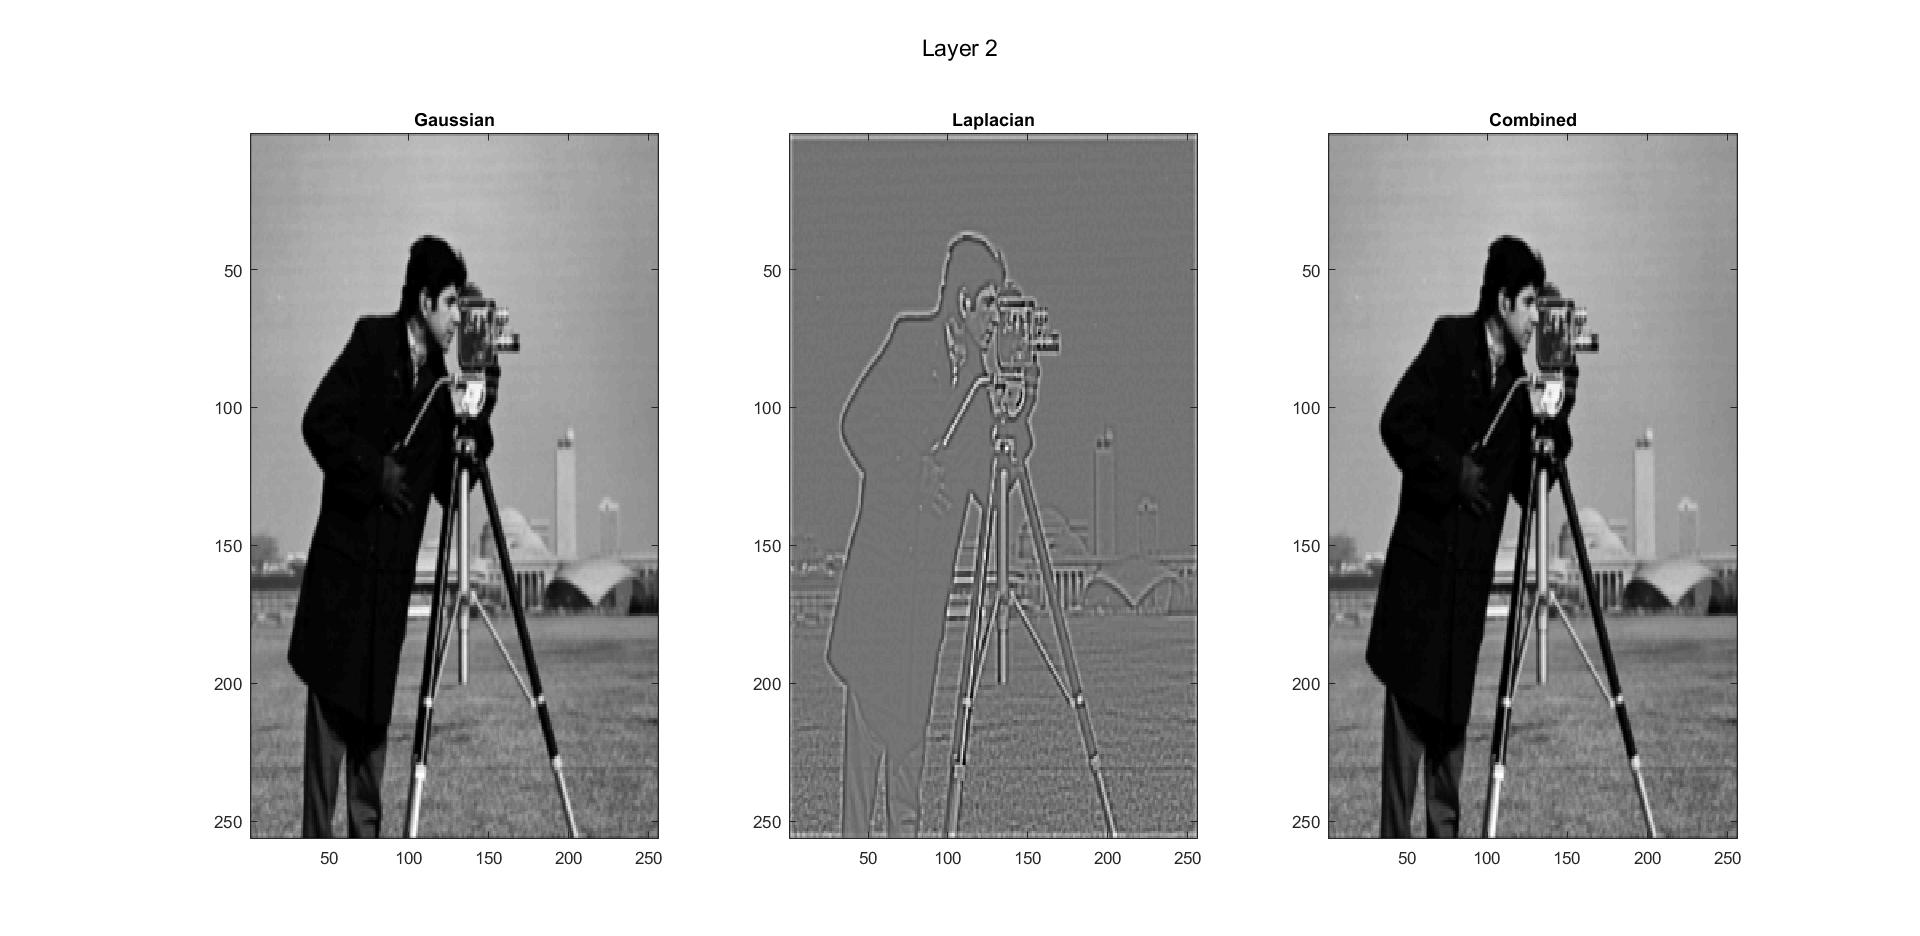
\includegraphics[width=\linewidth]{./output_images/layer_2.jpg}
			\caption{Gaussian and Laplacian pyramid and their compination - Layer 2}
		\end{subfigure}%
		
		\begin{subfigure}[t]{0.5\textwidth}
			\centering
			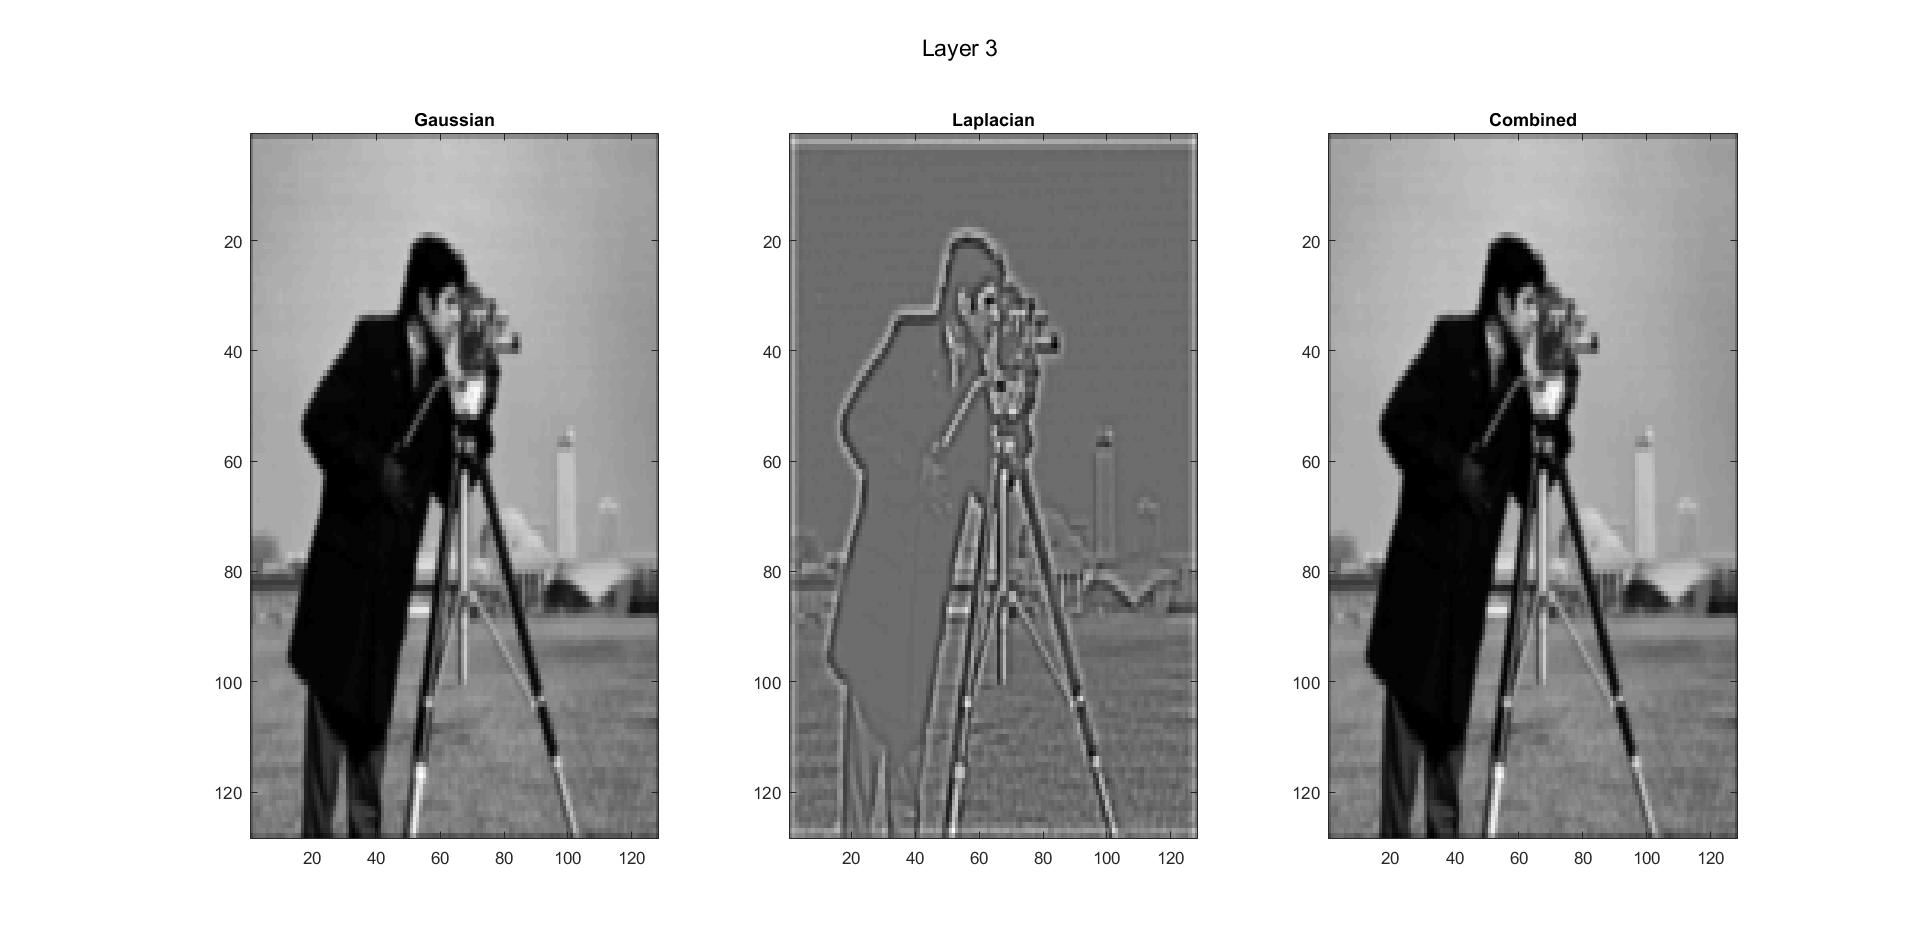
\includegraphics[width=\linewidth]{./output_images/layer_3.jpg}
			\caption{Gaussian and Laplacian pyramid and their compination - Layer 3}
		\end{subfigure}%
		~
		\begin{subfigure}[t]{0.5\textwidth}
			\centering
			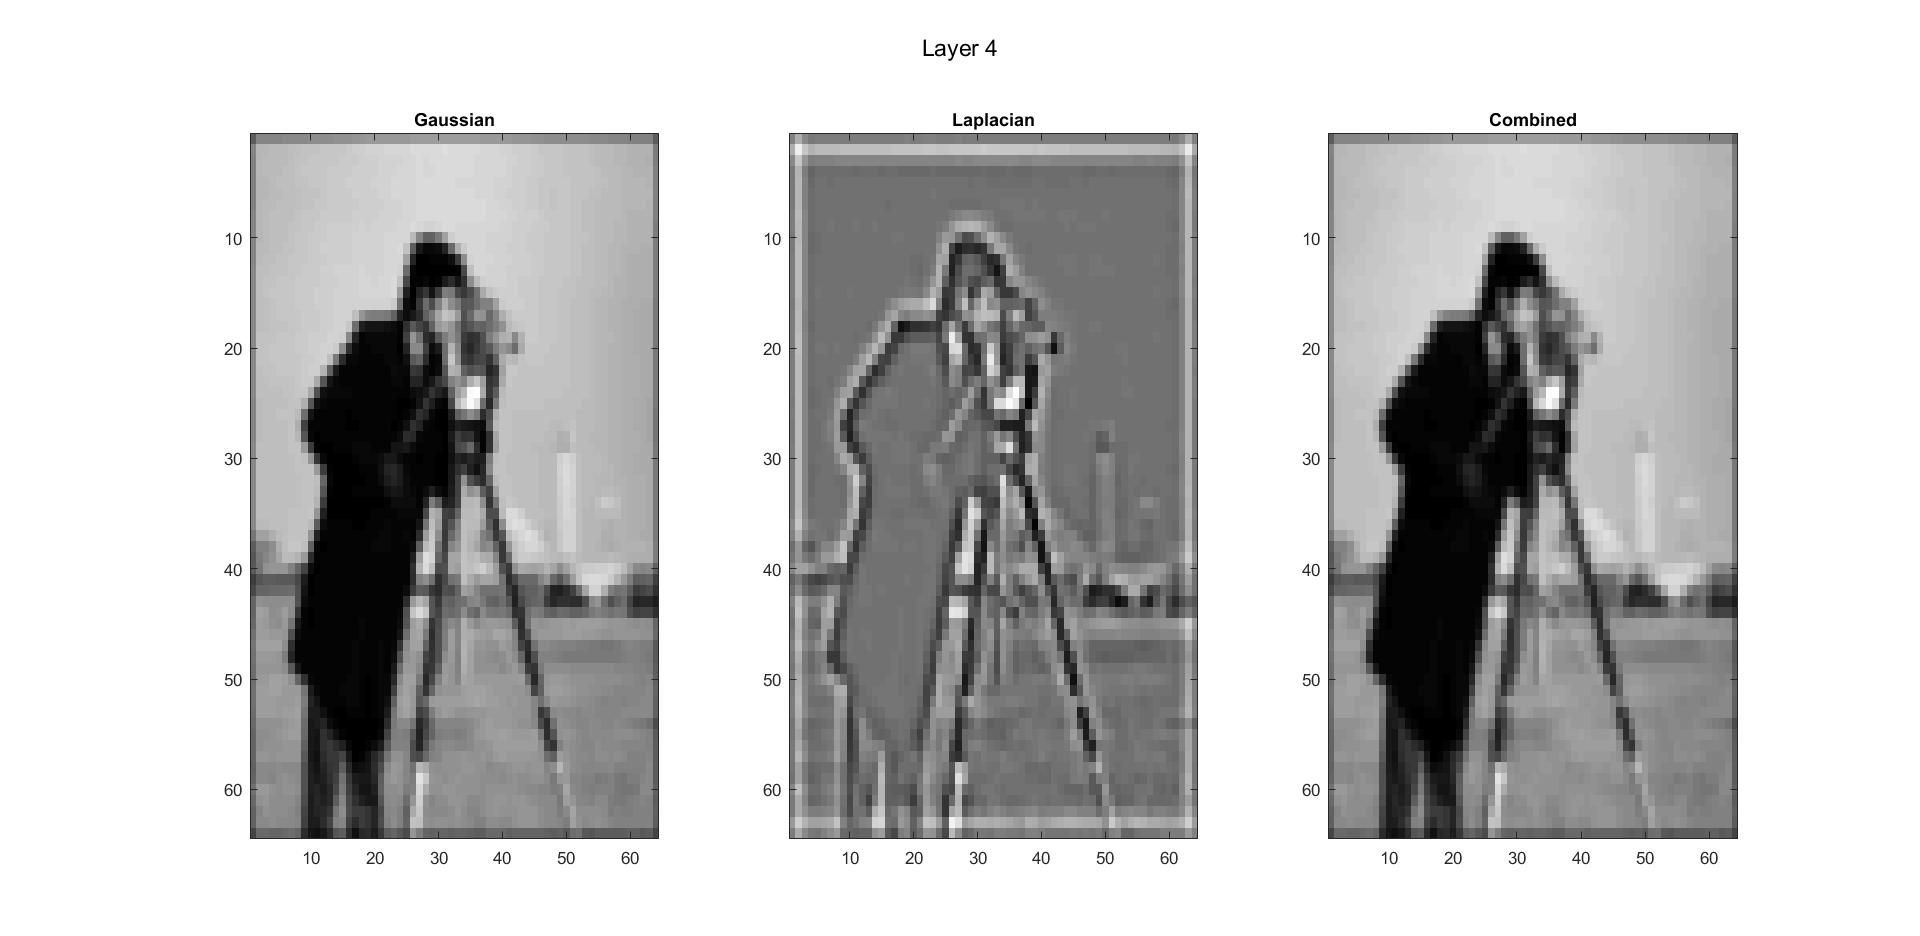
\includegraphics[width=\linewidth]{./output_images/layer_4.jpg}
			\caption{Gaussian and Laplacian pyramid and their compination - Layer 4}
		\end{subfigure}%
		
		\begin{subfigure}[t]{0.5\textwidth}
			\centering
			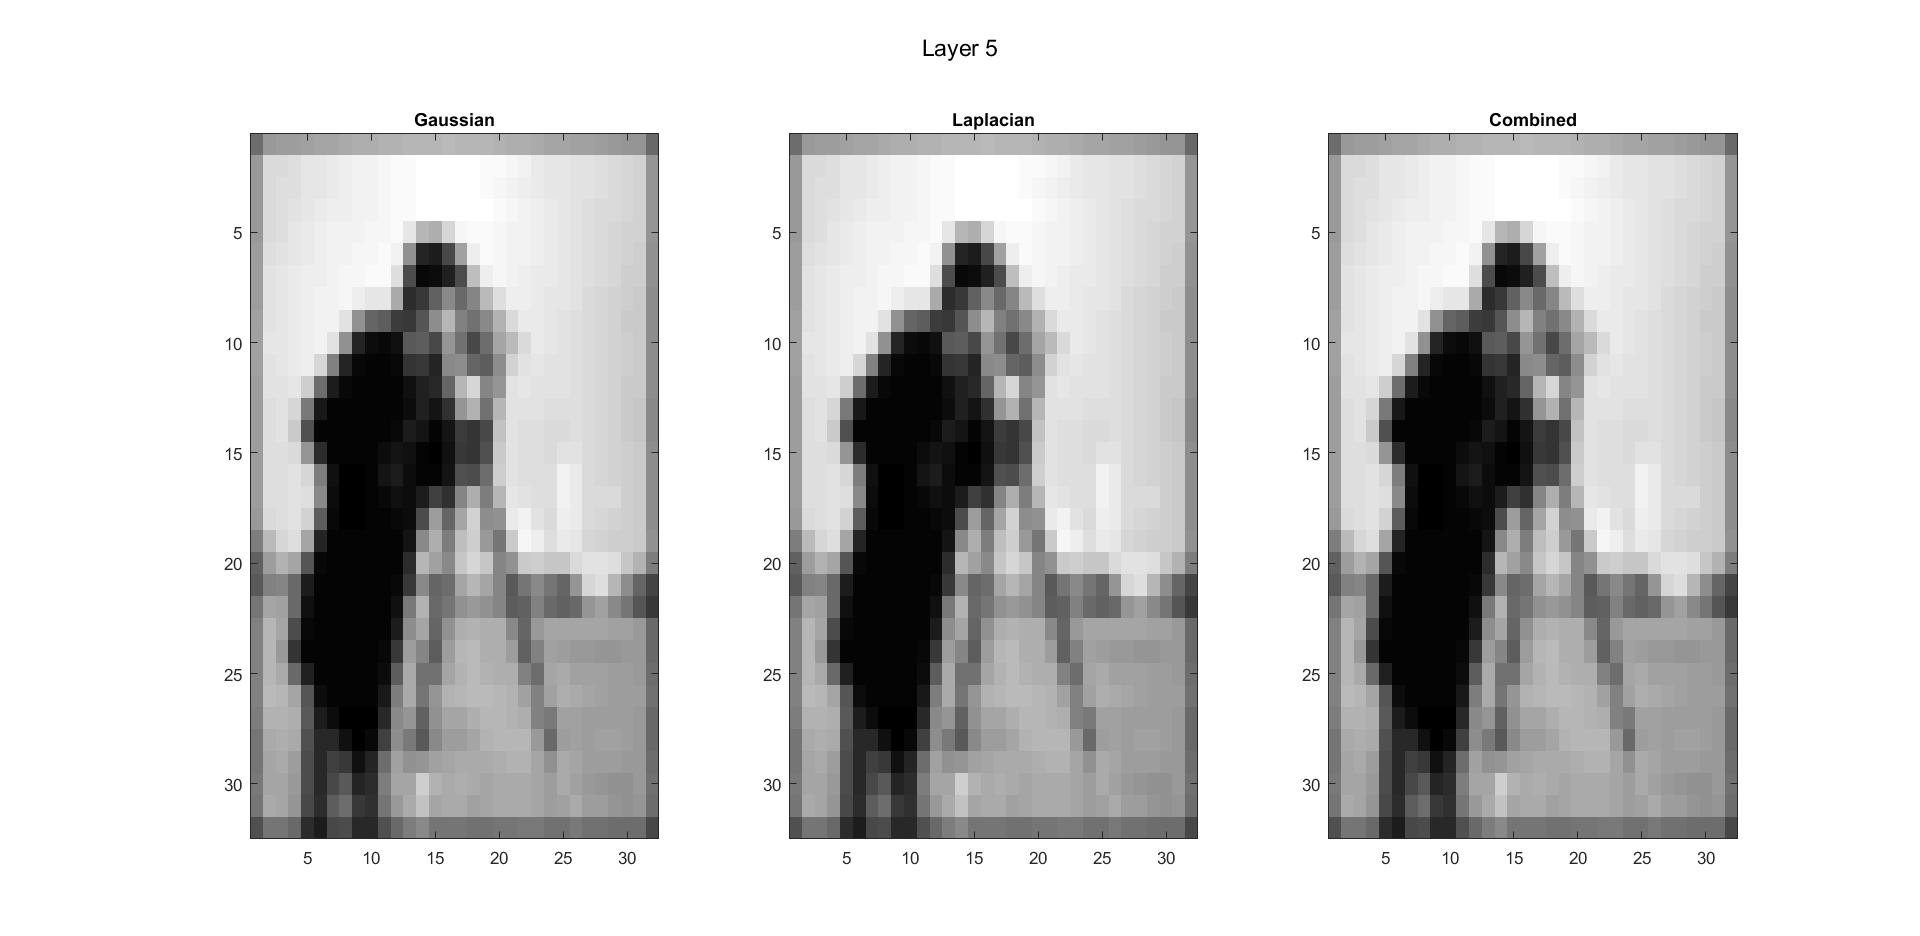
\includegraphics[width=\linewidth]{./output_images/layer_5.jpg}
			\caption{Gaussian and Laplacian pyramid and their compination - Layer 5}
		\end{subfigure}		
	\end{figure}
\end{document}
